\documentclass{article}
\usepackage[margin=1in]{geometry}
\usepackage{microtype}
\usepackage{setspace}
\usepackage{amsmath}
\usepackage{parskip}
\usepackage{amssymb}
\usepackage{graphicx}

\graphicspath{{../public/}}

\parskip=4ex
\date{}
\author{}

\title{11.3 Derivatives}

\begin{document}
  \maketitle
  \textbf{Notations}\\
  If $ \zstroke = f(x,y), $
  \[
    \begin{gathered}
    f_{x}(x,y)=f_{x}=\frac{\partial f}{\partial x}=\frac{\partial z}{\partial x} f(x,y) = D_1f = D_xf\\
    f_{y}(x,y)=f_{y}=\frac{\partial f}{\partial y}=\frac{d}{y} f(x,y)\\
    \frac{\partial dz}{\partial dy},~ f_{2},~,~D_{2}f,~D_{y}f    
    \end{gathered}
  \]

  \textbf{Rules for Finding Partial Derivatives}\\
  1) To find $ f_{x} $, regard $ y $ as a constant and differentiate $ f(x,y) $ with respect to x.

  2) To find $ f_{y}  $, regard $ y $ as a constant and differentiate $ f(x,y) $ with respect to y.

  \textbf{Ex 1}\\
  If $ f(x,y) =x^{3}+x^{2}y^{3}-2y^{2}    $, find $ f_{x}(2,1) ~\&~ f_{y}(2,1)$.
  \[
    \begin{gathered}
      f_{x}(x,y)= \frac{d}{dx}x^{3}+\frac{d}{dx}(x^{2}y^{3})-\frac{d}{dx}{2y^{2}}\\
      ~\\
      3x^{2}+  y^{3} \cdot \frac{d}{dx}x^{2}-0\to 3x^{2}+2xy^{3}\\
      ~\\
      f_{x}(2,1) = 3(2)^{2} + 2(2)(1)^{3}\to \boxed{16}\\
      ~\\
      f_{y}(x,y)= \frac{d}{dy}x^{3}+\frac{d}{dy}(x^{2}y^{3})-\frac{d}{dy}2y^{2}.      
    \end{gathered}
  \]

  \textbf{Interpretations of Partial Derivatives}\\
  A geometric interpretation of partial derivatives can be started with regarding that the equation $ f=f(x,y) $ represetns a surface $ S $ (the graph of f). If $ f(a,b) = c$, then the point $ P(a,b,c) $ lies on $ S $. By fixing $ y=b $, our attention is restricted to the curve $ C_1 $ in which the vertible plane $ y=b $ intersects $ S $. In other words, $ C_1 $ of $ S $ in the plane $ y=b $. Likewise, the vertical plane $ x=a $ intersects $ S $ in a curve $ C_2 $. Both of the curves $ C_1 ~\&~ C_2 $ pass through the point $ P $.
  
  \begin{center}
    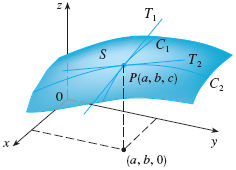
\includegraphics[width=8cm]{11_3_1}
  \end{center}
  The partial derivatives of $ f $ at $ (a,b) $ are the slopes of the tangents to $ C_1 ~\&~ C_2 $.

  The curve $ C_1 $ is the graph of the function $ g(x) = f(x,b) $, so the slope of its tangent $ T_1 $ at $ P $ is $ g'(a)=f_x(a,b) $. The curve $ C_2 $ is the graph of then function $ G(y)=f(a,y) $, so the slope of its tangent $ T_2 $ at $ P $ is $ G'(b)=f_y(a,b) $.

  Thus the partial derivatives of $ f_x(a,b) ~\&~ f_y(a,b) $ can be interpreted geometricaly as the slopes of the tangent lines at $ P(a,b,c) $ to the traces $ C_1 ~\&~ C_2 p $ of $ S $ in the planes $ y=b ~\&~ x=a $.

  Partial derivatives can also be interpreted as rates of change. If $ z=f(x,y) $, then $ \frac{\partial z}{\partial x} $ represents the rate of change of $ z $ with respect to $ x $ when $ y $ is fixed.

  \textbf{Ex 2}\\
  If $ f(x,y) = 4-x^{2} - 2y^{2} $, find $ f_x(1,1) ~\&~ f_y(1,1) $ and intepret these numbers as slopes.
  \[
    \begin{gathered}
    f_x(x,y) = -2x \qquad f_y(x,y)=-4y\\
    f_x(1,1)=-2  \qquad f_y(1,1)=-4
    \end{gathered}
  \]

  The graph of $ f $ is the paraboloid $ z=4-x^{2}-2y^{2} $ \& the verticle plane $ y=1 $ intersects it in the parabola $ z=2-x^{2},y=1 $, labeled $ C_1 $ (Top Figure) Then the slope of the tangent line to this parabola at the point $ (1,1,1) is f_x(1,1)=-2 $. Similarly, the curve $ C_2 $ in which the plane $ x=1 $ intersects the paraboloid is the parabola $ z=3-2y^{2},x=1 $ and the slope of the tangent line at $ (1,1,1) $ is $ f_y(1,1)=4 $ (Bottom Figure).
  \begin{center}
    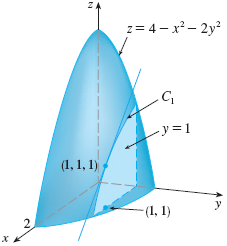
\includegraphics[width=8cm]{11_3_2}
  \end{center}
  \begin{center}
    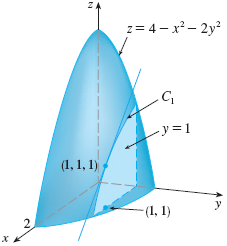
\includegraphics[width=8cm]{11_3_2}
  \end{center}
  
  \textbf{Ex 4}\\
Find $ \frac{\partial z}{\partial x} ~\&~ \frac{\partial z}{\partial y} $ if $ z $ is defined implicitly as a function of $ x ~\&~ y $ by the equation $ x^{3}+y^{3}+z^{3}+6xyz=1 $ 
 \[
   \begin{gathered}
   \frac{\partial z}{\partial x}\\
   ~\\
   3x^{2}+3z^{2}\frac{\partial z}{\partial x}+6yz+6xy=0\\
   ~\\
   \frac{\partial z}{\partial x}=-\frac{x^{2}+2yz}{z^{2}+2xv}\\
   ~\\
   \frac{\partial z}{\partial y}\\
   \frac{\partial z}{\partial v}=-\frac{y^{2}+2xz}{z^{2}+2xy}
   \end{gathered}
 \] 

\end{document}
